\documentclass[12pt]{article}
\usepackage{imakeidx} % Per creare un vero indice
\usepackage[italian]{babel}
\usepackage[utf8]{inputenc}
\usepackage[T1]{fontenc}
\usepackage{tikz}
\usepackage{float}
\usepackage{enumitem}
\usepackage{pifont}
\usepackage{xcolor}
\usepackage{graphicx}
\usepackage{hyperref}
\usepackage[margin=1in]{geometry}
\usepackage{eso-pic}
\usepackage{enumitem}
% Per gestire meglio la pagina
\usepackage{wallpaper}
\usepackage{graphicx} % Importa il pacchetto graphicx per l'inserimento di immagini
\usepackage{listings}
\usepackage[table]{xcolor}
\definecolor{darkblue}{rgb}{0.0, 0.0, 0.5} % Un blu scuro
\usepackage{colortbl}
\usepackage{xcolor}
\usepackage{listings}

%% Additional packages and commands
\usepackage{parskip}
\setlist{itemsep=-2pt} % Reducing white space in lists slightly
\renewcommand{\deg}{\si{\degree}\xspace} % Use \deg easily, everywhere

% Colore setting
\definecolor{deepblue}{RGB}{0,20,60}
% Definizione di una palette di colori sui toni del blu


% Configurazione dello stile per il codice (toni del blu)
\lstset{
	language=Python,            % Linguaggio del codice
	backgroundcolor=\color{blue!5}, % Sfondo leggermente azzurro
	frame=single,               % Bordo singolo attorno al codice
	rulecolor=\color{blue},     % Colore del bordo
	numbers=left,               % Numeri di riga a sinistra
	numberstyle=\tiny\color{blue!70}, % Stile dei numeri di riga
	basicstyle=\ttfamily\small, % Stile base del testo (monospace, piccolo)
	keywordstyle=\color{blue},  % Stile delle parole chiave
	commentstyle=\color{blue!70}, % Stile dei commenti
	stringstyle=\color{blue!50},  % Stile delle stringhe
	breaklines=true,            % Abilita la rottura delle righe lunghe
	tabsize=4                   % Dimensione dei tab
}

\makeindex % Attiva la creazione dell'indice
\begin{document}
	
	% Impostazione della numerazione delle pagine
	\pagenumbering{arabic}  % Imposta la numerazione delle pagine in numeri arabi
	
	% La numerazione inizia dalla prima pagina
	\pagestyle{empty}  % Imposta lo stile della pagina con la numerazione (senza intestazione)
	
	\begin{titlepage}
		% Inserisce l'immagine di sfondo
		\begin{tikzpicture}[remember picture,overlay]
			% Immagine di sfondo ridimensionata
			\node[inner sep=0pt] at (current page.center){
				\includegraphics[width=\paperwidth,height=\paperheight]{immagini/copertina2}
			};
			
			% Overlay colorato
			\fill[color=deepblue,opacity=0.8.5] 
			(current page.north west) -- 
			(current page.north east) -- 
			(current page.south east) -- 
			(current page.south west) -- 
			cycle;
		\end{tikzpicture}
		% Contenuto sovrapposto all'immagine
		\centering
		\vspace*{2cm}
		
		{\large\color{white}Dipartimento di Scienze Aziendali - Management \& Innovation Systems\\
			Corso di Laurea in Data Science \& Gestione dell'Innovazione\par}
		\vspace{0.8cm}
		
		{\Huge\color{white}\textbf{ Il Gabibbo: una figura controversa}\par}
		\vspace{1cm}
		
		{\Large\color{white} Come il Gabibbo ha creato un esercito di neofascisti nell'Italia del 21esimo secolo\par}
		\vspace{1.5cm}
		
		{\large\color{white}INFORMATION DISORDER AND GLOBAL SECURITY\par}
		\vspace{0.5cm}
		
		\vfill
		
	\end{titlepage}
	\newpage
	% Creazione della copertina
	\begin{titlepage}
		\centering
		\vspace*{1cm}
		
		% Titolo del report
		{\Huge \textbf{Echoes of the right: La genesi delle community altright su Telegram}}\\
		\vspace{0.5cm}
		{\LARGE Come i network digitali hanno forgiato l'altright su Telegram}\\
		\vspace{1.5cm}
		
		% Autore
		\textbf{by}\\
		\vspace{0.5cm}
		{\Large Denise Brancaccio - MAT. 0222800163}\\
		{\Large Lucia Brando - MAT. 0222800162}\\
		{\Large Bruno Maria Di Maio - MAT. 0222800149}
		\vspace{0.5cm}
		
		\vfill
		
		% Informazioni aggiuntive
		\textbf{Instructor:} G. Fenza \\
		\textbf{Teaching Assistant:} D. Cavaliere \\
		\textbf{Project Duration:} Month, Year -- Month, Year \\
		\textbf{Faculty:} Data Science \& Gestione dell'Innovazione \\
		\vspace{1cm}
		
		% Logo
		\includegraphics[width=0.3\textwidth]{immagini/logodisamis}\\
		\vspace{0.5cm}
		\vspace*{1cm}
	\end{titlepage}
	\newpage
	\pagestyle{plain}
	% Titolo della prefazione
	\begin{center}
		{\Large \begin{flushright}
				\textbf{Prefazione}
		\end{flushright}} % Titolo grande e in grassetto
	\end{center}
	
	\vspace{0.5cm} % Spazio verticale tra il titolo e il contenuto
	
	% Testo della prefazione
	\hspace{0.5cm} % Indentazione da sinistra
	\begin{flushleft}
		\textit{Il mondo delle community online ha assunto un ruolo sempre più centrale nella formazione delle opinioni, nella condivisione di informazioni e nella costruzione di identità collettive. \\Con la crescente diffusione di notizie false e la polarizzazione delle opinioni, è cruciale comprendere le dinamiche di queste community e il loro rapporto con la qualità delle fonti informative. \\Questo lavoro si propone di esplorare il livello di apertura delle community su Telegram e il legame tra tale apertura e l'attendibilità dei siti di notizie condivisi al loro interno. \\L'obiettivo è non solo mappare le connessioni tra le community e le fonti, ma anche fornire uno strumento di analisi visiva che evidenzi le dinamiche di interazione attraverso l'utilizzo di grafi generati con Gephi. \\Questo studio si inserisce in un contesto di ricerca multidisciplinare che combina data science, analisi delle reti sociali e valutazione delle fonti informative, offrendo nuove prospettive sulla comprensione dell'ecosistema informativo digitale.}
	\end{flushleft} % Testo in corsivo
	\vspace{0.5cm}
	
	
	\newpage
	\pagestyle{empty} % Disabilita numerazione e intestazioni
	\vspace*{\fill} % Riempie la pagina senza contenuti
	\thispagestyle{empty} % Assicura che anche questa pagina sia senza intestazione
	
	\newpage
	\renewcommand{\contentsname}{Indice} % Rinomina la tabella dei contenuti
	\tableofcontents % Genera la tabella dei contenuti
	\clearpage
	\section{Introduzione}
	\pagestyle{plain}
	\index{Introduzione}
	Negli ultimi anni, la diffusione di informazioni sui social media e sulle piattaforme di messaggistica istantanea ha radicalmente trasformato il modo in cui le persone accedono alle notizie.\\ 
	\textbf{Telegram}, in particolare, è emerso come uno degli strumenti più utilizzati per la condivisione di contenuti informativi, grazie alla sua flessibilità e alla capacità di ospitare gruppi e canali con migliaia di membri. Tuttavia, questa libertà d'uso si accompagna a rischi significativi, tra cui la proliferazione di notizie false e l'amplificazione di narrazioni manipolatorie.
	\\
	Le \textbf{community online} rappresentano un microcosmo di dinamiche sociali e informative, dove l'apertura – intesa come la capacità di interagire con fonti e utenti esterni – gioca un ruolo cruciale nel determinare la qualità e l'affidabilità delle informazioni condivise.\\ \textit{\textbf{Questo studio si propone di investigare il rapporto tra il livello di apertura delle community e l'attendibilità delle fonti giornalistiche che vi circolano, offrendo una panoramica approfondita delle interazioni tra utenti, contenuti e fonti informative}}.
	\subsection{Obiettivo principale}
	L'obiettivo principale di questo lavoro è analizzare il livello di apertura delle community presenti su Telegram e correlare tale apertura all'affidabilità dei siti di notizie condivisi.\\ Attraverso l'utilizzo di dati raccolti direttamente da \textbf{Telegram}, incrociati con valutazioni fornite da \textbf{NewsGuard}, si mira a costruire un grafo rappresentativo delle connessioni e delle interazioni tra community e fonti informative.\\
	Il grafo, realizzato tramite \textbf{Gephi}, consente una visualizzazione chiara e intuitiva delle dinamiche emerse, facilitando l'identificazione di pattern significativi e relazioni critiche.
	\newpage
	\section{Metodi e strumenti di lavoro}
	Per condurre l'analisi, è stato sviluppato uno \textbf{script Python} progettato per raccogliere dati da Telegram. 
	\\Questo script ha permesso di filtrare i messaggi contenenti link a siti di notizie. \\I dati raccolti sono stati elaborati confrontandoli con i punteggi di \textbf{NewsGuard}, generando così un file .csv che includeva nodi (le community) e archi (le connessioni tra essi). \\Il file è stato poi importato in \textbf{Gephi} per creare un grafo che rappresentasse visivamente le dinamiche informative.
	\subsection{Glossario}
		Di seguito si riportano alcuni dei termini chiave utilizzati nel contesto della comunicazione e della diffusione delle informazioni.\\
		Sono stati utilizzati termini che identificano contenuti di attualità e aggiornamenti di rilevante importanza:
	\begin{itemize}[label=\ding{109}] 
		\item News
		\item Breaking
		\item Alert
		\item Headline
		\item Update
		\item Broadcast
	\end{itemize}
	Termini che si riferiscono a diverse tipologie di documenti informativi e giornalistici:
	\begin{itemize}[label=\ding{109}] 
		\item Report
		\item Article
		\item Scoop
		\item Flash
		\item Bulletin
		\item Interview
	\end{itemize}
	Termini che indicano fenomeni informativi trasmessi in tempo reale o caratterizzati da una rapida diffusione:
	\begin{itemize}[label=\ding{109}] 
		\item Live
		\item Trending
		\item Viral
		\item Insight
		\item Timeline
		\item Profile
		\item Community
	\end{itemize}
	Termini che descrivono situazioni di urgenza o emergenza:
	\begin{itemize}[label=\ding{109}] 
		\item Emergency
		\item Incident
		\item Accident
		\item Disaster
		\item Crisis
	\end{itemize}
	Sono stati utilizzati, inoltre, temi di rilevanza sociale e politica:
	\begin{itemize}[label=\ding{109}] 
		\item Conflict
		\item War
		\item Pandemic
		\item Health
		\item Technology
		\item Economy
		\item Politics
		\item Elections
		\item Debate
		\item Protest
	\end{itemize}
	Ma anche termini che delineano strumenti, processi e dinamiche legati alla raccolta, elaborazione e diffusione dell’informazione:
	\begin{itemize}[label=\ding{109}] 
		\item Survey
		\item Poll
		\item Results
		\item Statistics
		\item Scandal
		\item Investigation
		\item Inquiry
		\item Revelation
		\item Discovery
		\item Press conference
		\item On Air
	\end{itemize}
	\subsection{Telegram}
	\begin{figure}[H]
		\centering
		\includegraphics[width=0.6\textwidth]{immagini/telegram}
	\end{figure}
	Telegram è una piattaforma di messaggistica molto utilizzata per la creazione di gruppi e canali tematici in cui gli utenti possono condividere e discutere contenuti.\\
	A differenza di altre piattaforme, Telegram permette la creazione di canali pubblici e gruppi con un numero potenzialmente illimitato di membri, favorendo una rapida diffusione delle informazioni. \\L'architettura di Telegram, infatti, consente agli utenti di condividere link a siti web, creando un ecosistema in cui notizie, articoli e contenuti virali possono diffondersi rapidamente. \\Questo lo rende un campo di studio ideale per analizzare la diffusione delle notizie, soprattutto in relazione alla qualità delle informazioni condivise. \\Inoltre, la disponibilità di API permette di raccogliere dati in modo automatizzato e strutturato, semplificando l'analisi dei messaggi e dei contenuti condivisi all'interno dei gruppi e canali. \\\textit{Per il nostro studio, Telegram è stato scelto come piattaforma principale per monitorare e raccogliere i dati, in quanto fornisce un ampio spettro di community diverse e informazioni su un vasto numero di argomenti, spesso trattati in modo non filtrato e senza verifica.}
	\subsection{NewsGuard}
	\begin{figure}[H]
	\centering
	\includegraphics[width=0.7\textwidth]{immagini/newsguard}
	\end{figure}
	NewsGuard è uno strumento che fornisce valutazioni affidabili sui siti web di notizie, assegnando loro un punteggio in base a criteri come la trasparenza, la correttezza e l'imparzialità dei contenuti. \\Ogni sito analizzato viene esaminato da un team di giornalisti professionisti, che valuta i parametri di qualità delle notizie pubblicate e fornisce una valutazione che aiuta gli utenti a discernere tra fonti affidabili e quelle che potrebbero diffondere disinformazione.\\ L'integrazione di NewsGuard nel nostro studio è stata essenziale, in quanto ha permesso di incrociare i link raccolti da Telegram con una valutazione professionale e oggettiva della loro affidabilità. \\
	\textit{Grazie a questo strumento, è stato possibile determinare se le fonti di notizie condivise all'interno delle community fossero credibili o se provenissero da siti tendenti alla disinformazione. \\L'utilizzo di NewsGuard ha aggiunto un ulteriore livello di analisi alla nostra ricerca, consentendo di classificare i dati in modo oggettivo e basato su criteri di qualità giornalistica.}
	\subsection{Gephi}
		\begin{figure}[H]
		\centering
		\includegraphics[width=0.6\textwidth]{immagini/gephilogo}
	\end{figure}
	Gephi è un software open-source utilizzato per l'analisi e la visualizzazione di grafi e reti complesse. \\È particolarmente utile per studiare le relazioni tra entità attraverso la rappresentazione visiva di nodi e archi, dove ogni nodo rappresenta un'entità (in questo caso, una community), mentre gli archi rappresentano le connessioni tra di esse. \\In questo studio, Gephi è stato utilizzato per visualizzare le connessioni tra i diversi nodi, permettendo una rappresentazione grafica che mostra la struttura e l'interconnessione di queste reti. \\L'importazione dei dati raccolti e strutturati in formato CSV ha consentito di generare un grafo interattivo che rende facilmente visibili le relazioni tra le community e le fonti di notizie, offrendo al contempo una panoramica immediata delle dinamiche di diffusione delle informazioni.\\ 
	\textit{Grazie alla sua capacità di gestire grandi quantità di dati e generare visualizzazioni dinamiche e interattive, Gephi ha svolto un ruolo cruciale nell'interpretazione e nella presentazione dei risultati, consentendo di osservare pattern, cluster e altre caratteristiche significative nelle connessioni tra le community e i siti di notizie.}
	\subsection{Open Measures}
	\begin{figure}[H]
		\centering
		\includegraphics[width=0.6\textwidth]{immagini/openmeasures}
	\end{figure}
	Open Measures è una piattaforma avanzata progettata per supportare l'analisi e il monitoraggio delle interazioni sui social media, con un focus particolare sui contenuti generati dagli utenti.\\
	La piattaforma offre API flessibili e potenti, che consentono di raccogliere dati strutturati su vasta scala.\\
	Questi dati includono messaggi, metadati (ad esempio, autore, data e ora), contenuti multimediali, e informazioni sulle relazioni tra utenti o entità.
	\\
	Le API di Open Measures sono progettate per essere altamente configurabili, permettendo di personalizzare le query attraverso parametri come parole chiave, intervalli temporali, e piattaforme social specifiche. Ciò consente agli utenti di accedere a dataset precisi e pertinenti per le loro analisi.\\ 
	Ad esempio, è possibile eseguire ricerche avanzate per identificare discussioni che menzionano URL, frasi chiave o hashtag, oppure per analizzare contenuti pubblicati su piattaforme come Telegram, Twitter o Reddit.
	\\
	Grazie alla sua architettura scalabile, Open Measures è particolarmente utile per progetti accademici, aziendali o governativi che richiedono l'analisi di grandi quantità di dati social.\\ 
	Le sue applicazioni spaziano dal monitoraggio della disinformazione e dell'hate speech, all'analisi dei trend, fino agli studi sull'engagement e sulla polarizzazione delle opinioni.\\ 
	Inoltre, la possibilità di esportare i dati in formati standard, come CSV, facilita l'integrazione con strumenti di analisi esterni come Python, R o software di visualizzazione come Gephi.
	\newpage
	\section{Sviluppo del lavoro}
	Il presente lavoro è articolato in diverse sezioni che riflettono il percorso di analisi intrapreso.\\
	Il seguente capitolo descriverà in dettaglio la metodologia adottata, illustrando le tecniche di raccolta, filtraggio e analisi dei dati.\\
	Il successivo capitolo presenterà i risultati ottenuti, con particolare attenzione alla mappatura delle community e alla visualizzazione dei grafi.\\
	Infine, verranno discussi i risultati evidenziando le implicazioni pratiche e teoriche, oltre a considerare i limiti dello studio e le potenziali direzioni future.
	\subsection{Raccolta e pre-analisi dei dati}
	La raccolta e la preparazione dei dati costituiscono la base fondamentale di questo studio, che mira ad analizzare il comportamento delle community su Telegram.\\
	In questa fase, è stata utilizzata una combinazione di strumenti di programmazione e dataset per strutturare le informazioni raccolte, filtrare i dati rilevanti e prepararli per l'analisi dei grafi.
	\subsubsection{File newsguard.csv}
	Per l'avvio del lavoro è stato utilizzato il file \textbf{"newsguard.csv"}, che contiene dati relativi a fonti di notizie.\\
	L'unico criterio applicato per filtrare i dati in fase iniziale è stato rappresentato dagli score assegnati alle fonti, variabili su una scala da 0 a 100.\\
	Questo approccio ha permesso di selezionare le fonti in base al loro punteggio senza ulteriori restrizioni.
	\begin{figure}[H]
		\centering
		\includegraphics[width=0.9\textwidth]{immagini/filtro.png}
	\end{figure}
	\subsubsection{File Open Measures.py}
	Per questo progetto è risultato fondamentale l'utilizzo dell'API di Open Measures.\\
	Grazie a quest'ultima, infatti, è stato possibile accedere a grandi quantità di dati strutturati relativi a Telegram, includendo metadati come contenuti dei messaggi, timestamp ed informazioni sugli autori.\\
	Per configurare il sistema, è necessario:
	\begin{itemize}[label=\ding{109}] 
		\item Ottenere un token di autorizzazione (salvato nel file \textbf{open-measures-key.txt}).
		\item Definire i parametri di ricerca attraverso file JSON (\textbf{parametri/terms.json}), che specificano le colonne richieste, i tipi di dati e i termini di ricerca. Ogni termine viene verificato: se è già stato processato, non viene ricercato nuovamente.
	\end{itemize}
	Un esempio di chiamata API con la funzione \textbf{fetch\_results} mostra la struttura del processo di raccolta:
	\begin{lstlisting}
		def fetch_results(term, social, start_date, end_date, attempt_count=None):
			if attempt_count is None:
				attempt_count = {"count": 1}
		
			current_attempt = attempt_count["count"]
		
			params = {
				'term': '(message:http OR message:https) AND message:%s' % term,
				'limit': 10000,
				'site': social,
				'since': start_date,
				'until': end_date,
				'esquery': 'true'
			}
	\end{lstlisting}
	La funzione genera query dinamiche per l’API, suddivide automaticamente gli intervalli temporali in caso di limiti di risultati, e converte le risposte in un DataFrame pandas.\\
	Quando il limite massimo di 10.000 risultati viene superato, l'intervallo temporale della query viene automaticamente suddiviso a metà.\\ Questo processo si ripete ricorsivamente fino a quando ogni intervallo produce meno di 10.000 risultati.
	\begin{lstlisting}
		...
		if len(hits) == 10000:
		mid_date = pd.Timestamp(start_date) + (pd.Timestamp(end_date) - pd.Timestamp(start_date)) / 2
		...
		first_half_df = fetch_results(term, social, start_date, mid_date, attempt_count)
		second_half_df = fetch_results(term, social, second_half, end_date, attempt_count)
		...
		else:
		df = pd.DataFrame([hit['_source'] for hit in hits])
		return df
	\end{lstlisting}
	Questa funzione suddivide gli intervalli temporali finché i dati non sono gestibili, garantendo una raccolta completa e robusta.\\
	Infine, i risultati sono stati salvati in file CSV per ogni termine analizzato, come mostrato nel seguente frammento di codice:
	\begin{lstlisting}
		output_file = "csv/social_termine_2024.csv"
		df.to_csv(output_file, index=False)
	\end{lstlisting}
	Questa metodologia ha garantito la scalabilità del processo di raccolta e la creazione di una base dati robusta per le successive fasi di analisi.\\
	I file finali generati sono in formato CSV e includono:
	\begin{itemize}
		\item \textbf{Colonne strutturate:} metadati come timestamp, contenuto dei messaggi, autori, ecc.
		\item \textbf{Dati consistenti:} grazie alla conversione automatica dei tipi di dati specificati nel file \textbf{dtypes.json}.
	\end{itemize}
	\textbf{\textit{Un termine come "disinformazione", ricercato su Telegram per gennaio 2024, ha prodotto dati relativi a messaggi contenenti URL (message:http OR message:https) e salvati nel file CSV corrispondente. Grazie all'automazione, ogni intervallo temporale è stato gestito in modo autonomo, senza intervento manuale.}}
	\subsubsection{File main.py}
	Il sistema presentato analizza messaggi provenienti da Telegram per individuare e filtrare URL che puntano a domini di interesse, forniti da un file di riferimento (Newsguard).\\
	Il processo include la lettura, il filtraggio e l'aggregazione dei dati in due output principali: \textbf{output.csv}, che raccoglie i messaggi rilevanti, e \textbf{occorrenze.csv}, che riassume statistiche di dominio.\\
	Gli obiettivi del sistema sono:
	\begin{itemize}[label=\ding{109}]
		\item Identificare i domini di interesse nei messaggi di Telegram
		\item Analizzare quantitativamente il numero di occorrenze, visualizzazioni (views) e inoltri (forwards)
		\item Generare output strutturati e pronti per analisi successive
	\end{itemize}
	Gli URL vengono estratti dai messaggi tramite la funzione \textbf{extract\_urls}, che normalizza i formati non standard (es. \textbf{[DOT] → .}) e identifica gli URL.
	\begin{lstlisting}
		def extract_urls(text):
		url_pattern = r"https?://(?:[-\w.]|(?:%[\da-fA-F]{2}))+"
		if isinstance(text, str):
		cleaned_message = re.sub(r"\[(DOT|dot|\.)\]", ".", str(text))
		cleaned_message = re.sub(r"\](?=\s|$)", "", cleaned_message)
		return re.findall(url_pattern, cleaned_message)
		return []
	\end{lstlisting}
	I domini vengono estratti dagli URL utilizzando la \textbf{libreria urllib}.parse per separare la parte rilevante.
	\begin{lstlisting}
		def extract_domain(url):
		try:
		parsed_url = urlparse(url)
		domain = parsed_url.netloc
		if domain.startswith("www."):
		domain = domain[4:]
		return domain.lower()
		except:
		return ""
	\end{lstlisting}
	La funzione\textbf{ process\_csvs} analizza i file CSV nella \textbf{directory csv/} e li confronta con i domini di interesse presenti nel file Newsguard.
	\begin{lstlisting}
		def process_csvs(output_filename, occorrenze_filename, newsguard_filename="Newsguard.csv", folder_path="csv"):
		newsguard_df = pd.read_csv(newsguard_filename).dropna(subset=["Score"]).drop_duplicates()
		
		original_domains = {domain.lower(): domain for domain in newsguard_df["Domain"] if isinstance(domain, str)}
		domain_scores = {domain.lower(): score for domain, score in zip(newsguard_df["Domain"], newsguard_df["Score"]) if isinstance(domain, str)}
		domain_orientations = {domain.lower(): orientation for domain, orientation in zip(newsguard_df["Domain"], newsguard_df["Orientation"]) if isinstance(domain, str)}
		
		newsguard_domains = set(original_domains.keys())
		columns_to_keep = ["message", "channelusername", "reactions", "forwards", "postauthor", "replies", "views"]
		
		matching_rows = []
		domain_stats = defaultdict(lambda: {"occorrenze": 0, "views": 0, "forwards": 0})
		
		for filename in os.listdir(folder_path):
		if filename.endswith(".csv"):
		print("Elaborazione file: %s" % filename)
		try:
		df = pd.read_csv(os.path.join(folder_path, filename), low_memory=False).drop_duplicates()
		for _, row in df.iterrows():
		if isinstance(row["message"], str):
		urls = extract_urls(row["message"])
		domains = {extract_domain(url) for url in urls}
		matching_domains = domains & newsguard_domains
		if matching_domains:
		matching_rows.append(row[columns_to_keep])
		views = int(row["views"]) if pd.notna(row["views"]) else 0
		forwards = int(row["forwards"]) if pd.notna(row["forwards"]) else 0
		for domain in matching_domains:
		domain_stats[domain]["occorrenze"] += 1
		domain_stats[domain]["views"] += views
		domain_stats[domain]["forwards"] += forwards
		except Exception as e:
		print("Errore nel processare %s: %s" % (filename, str(e)))
		
		if matching_rows:
		output_df = pd.DataFrame(matching_rows)
		output_df.to_csv(output_filename, index=False)
		print("\nAnalisi completata. File %s creato con %s corrispondenze." % (output_filename, len(output_df)))
		else:
		print("\nNessuna corrispondenza trovata.")
		
		occorrenze_data = []
		for domain_lower, stats in domain_stats.items():
		if stats["occorrenze"] > 0:
		occorrenze_data.append({
			"Domain": original_domains[domain_lower],
			"Score": domain_scores[domain_lower],
			"Orientation": domain_orientations[domain_lower],
			"Occorrenze": stats["occorrenze"],
			"Views": stats["views"],
			"Forwards": stats["forwards"]
		})
		
		if occorrenze_data:
		occorrenze_df = pd.DataFrame(occorrenze_data)
		occorrenze_df = occorrenze_df.sort_values("Occorrenze", ascending=False)
		occorrenze_df.to_csv(occorrenze_filename, index=False)
		print("File %s creato con %s domini attivi.\n" % (occorrenze_filename, len(occorrenze_df)))
		else:
		print("Nessun dominio con occorrenze trovato.\n")
	\end{lstlisting}
	Le tipologie di output che si ottengono sono le seguenti:
	\begin{itemize}[label=\ding{109}]
		\item \textbf{output.csv:} Fornisce una visione dettagliata dei messaggi corrispondenti, utile per analisi qualitative e per approfondire il contesto dei domini rilevati.
		\item \textbf{occorrenze.csv:} Riassume i dati quantitativi, ordinando i domini per numero di occorrenze in ordine decrescente, evidenziando i domini più rilevanti.
		\begin{table}[h!]
			\centering
			\renewcommand{\arraystretch}{1.5}
			\setlength{\tabcolsep}{12pt}
			\rowcolors{2}{gray!10}{white}
			\begin{tabular}{|c|c|c|c|c|c|}
				\hline
				\rowcolor{darkblue!80} \textcolor{white}{\textbf{Domain}} & \textcolor{white}{\textbf{Score}} & \textcolor{white}{\textbf{Orientation}} & \textcolor{white}{\textbf{Occorrenze}} & \textcolor{white}{\textbf{Views}} & \textcolor{white}{\textbf{Forwards}} \\ \hline
				dominio1.com & 60 & Neutral & 120 & 1500 & 300 \\ \hline
				dominio2.com & 90 & Left   & 75  & 800  & 120 \\ \hline
				dominio3.com & 40 & Right  & 45  & 500  & 100 \\ \hline
			\end{tabular}
		\end{table}
	\end{itemize}
	\subsubsection{File gephi.py}
	Il file gephy.py è uno script che processa i dati presenti nel file output.csv per generare due file output:
	\begin{itemize}[label=\ding{109}]
		\item \textbf{nodes.csv:} contiene l'elenco dei nodi ed il loro tipo
		\item \textbf{archs.csv:} contiene le relazioni tra i nodi
	\end{itemize}
	Questi file sono progettati per essere compatibili con Gephi e rappresentano rispettivamente i nodi (utenti e canali) e le relazioni (interazioni) tra di essi.
	Lo script ha lo scopo di:
	\begin{itemize}[label=\ding{109}]
		\item \textbf{Identificare i nodi:} creare un elenco di utenti e canali
		\item \textbf{Generare le relazioni:} costruire gli archi che rappresentano interazioni, come risposte tra utenti e canali
		\item \textbf{Salvare i risultati}
	\end{itemize}
	Lo script si articola in quattro sezioni principali.\\
	La prima è la lettura del file \textbf{output.csv}:
	\begin{lstlisting}
		# Lettura del file CSV
		data = pd.read_csv("output.csv")
		df = pd.DataFrame(data)
	\end{lstlisting}
	Per ogni riga del file, lo script analizza la \textbf{colonna replies}, che contiene le informazioni sugli utenti che hanno risposto a un determinato canale.\\
	Se la colonna \textbf{replies} è un dizionario valido, vengono estratti gli identificatori univoci degli utenti (\textbf{user\_id}) e i canali a cui hanno risposto.\\
	Questi dati vengono salvati nel dizionario \textbf{dizionario}.
	\begin{lstlisting}
		dizionario = {}
		
		for index, replies in enumerate(df["replies"]):
		# Converti la stringa in un dizionario
		if isinstance(replies, str):
		replies = ast.literal_eval(replies)
		if isinstance(replies, dict) and replies["recent_repliers"]:
		for user, _ in enumerate(replies["recent_repliers"]):
		# Estrai l'ID dell'utente
		if "user_id" in replies["recent_repliers"][user]:
		user_id = replies["recent_repliers"][user]["user_id"]
		channel = df["channelusername"][index]
		# Aggiungi l'utente e il canale al dizionario
		if user_id not in dizionario:
		dizionario[user_id] = ("User", [channel])
		else:
		dizionario[user_id][1].append(channel)
	\end{lstlisting}
	I dati elaborati, come già detto in precedenza vengono salvati in due file csv.
	\subsubsection{File node.csv:}
	\begin{lstlisting}
		nodes = "nodes.csv"
		target_set = set()
		
		with open(nodes, mode="w", newline="", encoding="utf-8") as file:
		writer = csv.writer(file)
		writer.writerow(["id", "type"])  # Intestazione
		
		for key, (value, target) in dizionario.items():
		writer.writerow([key, value])  # Nodo utente
		for element in target:
		if element not in target_set:
		target_set.add(element)
		writer.writerow([element, "Channel"])  # Nodo canale
	\end{lstlisting}
	\begin{table}[h!]
		\centering
		\renewcommand{\arraystretch}{1.5}
		\setlength{\tabcolsep}{12pt}
		\rowcolors{2}{gray!10}{white}
		\begin{tabular}{|p{6cm}|p{8cm}|}
			\hline
			\cellcolor{darkblue}\textcolor{white}{\textbf{ID}} & \cellcolor{darkblue}\textcolor{white}{\textbf{Type}} \\
			\hline
			\textbf{12345678} & User \\
			\hline
			\textbf{channel\_1} & Channel\\
			\hline
		\end{tabular}
	\end{table}
	\newpage
	\subsubsection{File archs.csv:}
	\begin{lstlisting}
		archs = "archs.csv"
		
		with open(archs, mode="w", newline="", encoding="utf-8") as file:
		writer = csv.writer(file)
		writer.writerow(["source", "target", "type"])  # Intestazione
		
		for key, (_, target) in dizionario.items():
		for element in target:
		writer.writerow([key, element, "Reply"])  # Arco tra utente e canale
	\end{lstlisting}
	\begin{table}[h!]
		\centering
		\renewcommand{\arraystretch}{1.5}
		\setlength{\tabcolsep}{12pt}
		\rowcolors{2}{gray!10}{white}
		\begin{tabular}{|p{5cm}|p{4cm}|p{4cm}|}
			\hline
			\cellcolor{darkblue}\textcolor{white}{\textbf{Source}} & 
			\cellcolor{darkblue}\textcolor{white}{\textbf{Target}} & 
			\cellcolor{darkblue}\textcolor{white}{\textbf{Type}} \\
			\hline
			\textbf{12345678} & channel\_1 & Reply \\
			\hline
		\end{tabular}
	\end{table}
	\subsubsection{File connections.py}
	Il file \textbf{connections.py} è una componente essenziale del progetto che estende le relazioni presenti nel dataset \textbf{archs.csv}.\\
	Il suo scopo è generare nuove connessioni tra i nodi basandosi su combinazioni esistenti e consolidare tali relazioni in un uovo file csv denominato \textbf{archs\_new.csv}.\\
	Lo script esegue le seguenti operazioni:
	\begin{itemize}[label=\ding{109}]
		\item \textbf{Caricamento del dataset originale:} utilizza il file archs.csv come input per leggere le connessioni esistenti
		\item \textbf{Raggruppamento per origine:} per ogni nodo sorgente, individua i nodi destinazione collegati (source->target)
		\item \textbf{Generazione di combinazioni:} crea tutte le possibili coppie tra i nodi di destinazione collegati a una stessa sorgente
		\item \textbf{Consolidamento delle connessioni:} concatena le connessioni generate con quelle originali e salva il risultato in \textbf{archs\_new.csv}
	\end{itemize}
	La prima parte del codice legge il dataset per manipolare i dati tabulari:
	\begin{lstlisting}
		import pandas as pd
		from itertools import combinations
		
		# Leggi il file
		df = pd.read_csv("archs.csv")
	\end{lstlisting}
	Il file \textbf{archs.csv} contiene le connessioni esistenti, strutturate con colonne \textbf{source, target e type}, dove:
	\begin{itemize}[label=\ding{109}]
		\item \textbf{Source:} rappresenta il nodo sorgente
		\item \textbf{Target:} rappresenta il nodo destinazione
		\item \textbf{Type:} specifica la natura della relazione
	\end{itemize}
	Successivamente, si va ad inizializzare le strutture per le nuove connessioni:
	\begin{lstlisting}
		# Nome del file di output
		output_file = "archs_new.csv"
		
		# Inizializza un DataFrame vuoto
		df_total_channels = pd.DataFrame(columns=["source", "target", "type"])
	\end{lstlisting}
	Lo script raggruppa i dati per source, estraendo per ciascun nodo sorgente l'elenco dei nodi di destinazioni associati.\\
	Successivamente, utilizza la \textbf{funzione combinations} della \textbf{libreria itertools} per generare tutte le coppie possibili tra questi nodi di destinazione:
	\begin{lstlisting}
		for _, group in df.groupby("source"):
		# Crea un set di utenti per evitare duplicati
		targets = set(group["target"])
		
		# Genera le combinazioni
		pairs = list(combinations(targets, 2))
		df_new = pd.DataFrame(pairs, columns=["source", "target"]).drop_duplicates()
		
		# Aggiungi la colonna "type" con valore "Connection"
		df_new["type"] = "Connection"
		
		# Concatena al DataFrame totale
		df_total_channels = pd.concat([df_total_channels, df_new], ignore_index=True)
	\end{lstlisting}
	In questo processo i nodi di destinazione vengono memorizzati in un set \textbf{(targets)} per garantire l'unicità e le combinazioni di coppie vengono generate per creare nuove connessioni indirette tra i nodi.\\
	Le connessioni aggiuntive vengono unite a quelle originali presenti nel dataset:
	\begin{lstlisting}
		# Concatena il DataFrame totale al DataFrame originale
		df_final = pd.concat([df, df_total_channels], ignore_index=True).dropna()
		df_final.to_csv(output_file, index=False)
	\end{lstlisting}
	Il risultato è salvato in un nuovo file \textbf{archs\_new.csv} che contiene sia le connessioni originali sia quelle derivate.
	\begin{table}
		\begin{tabular}{|p{5cm}|p{4cm}|p{4cm}|}
			\hline
			\cellcolor{darkblue}\textcolor{white}{\textbf{Source}} & 
			\cellcolor{darkblue}\textcolor{white}{\textbf{Target}} & 
			\cellcolor{darkblue}\textcolor{white}{\textbf{Type}} \\
			\hline
			\textbf{user123} & canale\_1 & Reply \\
			\hline
			\textbf{user123} & canale\_2 & Reply\\
			\hline
			\textbf{user456} & canale\_3 & Reply\\
		\end{tabular}
		\caption{Esempio di file `archs.csv`.}
		\label{tab:archs.csv}
	\end{table}
	\begin{table}
		\begin{tabular}{|p{5cm}|p{4cm}|p{4cm}|}
			\hline
			\cellcolor{darkblue}\textcolor{white}{\textbf{Source}} & 
			\cellcolor{darkblue}\textcolor{white}{\textbf{Target}} & 
			\cellcolor{darkblue}\textcolor{white}{\textbf{Type}} \\
			\hline
			\textbf{user123} & canale\_1 & Reply \\
			\hline
			\textbf{user123} & canale\_2 & Reply\\
			\hline
			\textbf{user456} & canale\_3 & Reply\\
			\hline
			\textbf{canale\_1} & canale\_2 & Connection\\
		\end{tabular}
		\caption{Esempio di file `archs\_new.csv` con connessioni derivate.}
		\label{tab:archs_new}
	\end{table}
	\newpage
	\subsubsection{File closure.py}
	In questa sezione verrà analizzato e descritto nel dettaglio il codice sviluppato per calcolare un indice denominato \textit{\textbf{"tasso di chiusura"}} per diverse community, andandosi a basare sulle interazioni tra utenti.
	Iniziamo con il caricare i dati:
	\begin{lstlisting}
		df = pd.read_csv("archs_new_2.csv")
		df = df[df.type == "Reply"]
		df_community = pd.read_csv("community.csv")
	\end{lstlisting}
	\begin{itemize}[label=\ding{109}]
		\item \textbf{archs\_new\_2.csv:} contiene informazioni sulle interazioni tra utenti, inclusi i tipi di messaggi inviati. Solo i messaggi di tipo "Reply" vengono considerati per le successive analisi.
		\item \textbf{community.csv:} fornisce dettagli sulle community, come il numero di messaggi e attributi associati.
	\end{itemize}
	I file csv vengono caricati in due dataframe denominati \textbf{df} e \textbf{df\_community}.\\
	Si prosegue, poi, con il calcolo degli utenti per canale:
	\begin{lstlisting}
		users_per_channel = df.groupby("target")["source"].apply(set).to_dict()
	\end{lstlisting}
	Questo passaggio raggruppa i dati in base ai canali destinatari \textbf{(target)} e crea un dizionario in cui ogni chiave rappresenta un canale, mentre il valore è l'insieme degli utenti \textbf{(source)}che hanno interagito con quel canale.\\
	Si passa al calcolo dei canali per utente:
	\begin{lstlisting}
		channels_per_user = df.groupby("source")["target"].apply(set).to_dict()
	\end{lstlisting}
	In modo simile, questo codice calcola per ogni utente l'insieme dei canali \textbf{(target)} con cui ha interagito. Il risultato è un dizionario in cui la chiave è un utente e il valore è un insieme di canali.\\
	Si calcola, poi, il tasso di chiusura:
	\begin{lstlisting}
		closure_scores = {}
		for channel, users in users_per_channel.items():
		total_channels = sum(len(channels_per_user[user]) for user in users)
		closure_scores[channel] = len(users) / total_channels
	\end{lstlisting}
	Quest'ultimo si tratta di una metrica che quantifica la concentrazione degli utenti in un canale rispetto al numero totale di canali con cui interagiscono. Per ogni canale:
	\begin{lstlisting}
		closure_scores = {}
		for channel, users in users_per_channel.items():
		total_channels = sum(len(channels_per_user[user]) for user in users)
		closure_scores[channel] = len(users) / total_channels
	\end{lstlisting}
	\begin{itemize}[label=\ding{109}]
		\item Si somma il numero di canali associati a ciascun utente del canale corrente
		\item Il tasso di chiusura è definito come il rapporto tra il numero di utenti unici del canale e il numero totale di canali con cui questi utenti interagiscono
	\end{itemize}
	Ultimo passo è l'integrazione del tasso di chiusura precedentemente calcolato:
	\begin{lstlisting}
		df_community["Tasso di chiusura"] = df_community["Community"].map(closure_scores)
	\end{lstlisting}
	I valori calcolati vengono mappati al DataFrame \textbf{df\_community}, aggiungendo una nuova colonna denominata "Tasso di chiusura".\\
	Solo le community che hanno almeno 200 messaggi vengono considerate:
	\begin{lstlisting}
		df_community = df_community[df_community["Messaggi"] >= 200].dropna(subset=["Tasso di chiusura"])
	\end{lstlisting}
	I dati filtrati e arricchiti con il tasso di chiusura vengono salvati in un nuovo file csv denominato \textbf{community\_new.csv}.
	\subsubsection{File community.py}
	In questo paragrafo finale, si va ad analizzare in dettaglio il codice sviluppato per l'elaborazione e l'analisi dei dati delle community, esaminando ogni componente e la sua funzione specifica nel processo complessivo.\\
	Il codice inizia con l'importazione delle librerie necessarie:
	\begin{itemize}[label=\ding{109}]
		\item\textbf{ pandas:} per la manipolazione dei dataframe.
		\item \textbf{re:} per le operazioni con espressioni regolari.
		\item \textbf{defaultdict:} per la gestione di dizionari con valori predefiniti.
		\item \textbf{urlparse:} per l'analisi degli URL.
		\item \textbf{numpy:} per operazioni numeriche efficienti
	\end{itemize}
	Il codice definisce anche alcuni pattern regex ottimizzati per il parsing degli URL e la pulizia del testo:
	\begin{lstlisting}
		URL_PATTERN = re.compile(r"https?://(?:[-\w.]|(?:%[\da-fA-F]{2}))+")
		DOT_PATTERN = re.compile(r"\[(DOT|dot|\.)\]")
		BRACKET_PATTERN = re.compile(r"\](?=\s|$)")
	\end{lstlisting}
	La funzione \textbf{preprocess\_newsguard\_data} si occupa di preparare i dati di Newsguard per l'analisi successiva:
	\begin{lstlisting}
		def preprocess_newsguard_data(newsguard_df):
		clean_df = newsguard_df.dropna(subset=["Score"]).drop_duplicates()
		
		return {
			'original_domains': {d.lower(): d for d in clean_df["Domain"] 
				if isinstance(d, str)},
			'orientations': {d.lower(): o for d, o in zip(clean_df["Domain"], clean_df["Orientation"]) 
				if isinstance(d, str)},
			'scores': {d.lower(): s for d, s in zip(clean_df["Domain"], clean_df["Score"])
				if isinstance(d, str)},
			'topics': {d.lower(): t for d, t in zip(clean_df["Domain"], clean_df["Topics"]) 
				if isinstance(d, str)}
		}
	\end{lstlisting}
	Questa funzione:
	\begin{itemize}[label=\ding{109}]
		\item Rimuove le righe con score mancanti e duplicati
		\item Crea quattro dizionari normalizzati per domini, orientamenti, score e topic
		\item Converte tutti i domini in minuscolo per garantire confronti case-insensitive
		\item Filtra eventuali valori non stringa per evitare errori
	\end{itemize}
	Le funzioni \textbf{extract\_urls} e \textbf{extract\_domain} lavorano in tandem per processare gli URL nei messaggi:
	\begin{lstlisting}
		def extract_urls(text):
		if not isinstance(text, str):
		return []
		cleaned = DOT_PATTERN.sub(".", text)
		cleaned = BRACKET_PATTERN.sub("", cleaned)
		return URL_PATTERN.findall(cleaned)
		
		def extract_domain(url):
		try:
		parsed = urlparse(url)
		domain = parsed.netloc
		return domain[4:].lower() if domain.startswith("www.") else domain.lower()
		except:
		return ""
	\end{lstlisting}
	Queste funzioni hanno gli scopi di:
	\begin{itemize}[label=\ding{109}]
		\item Normalizzano il testo sostituendo varianti di "dot" con punti
		\item Estraggono tutti gli URL validi dal testo
		\item Parsano gli URL per estrarre domini
		\item Rimuovono il prefisso "www." e convertono in minuscolo
	\end{itemize}
	Il vero cuore dell'analisi è la funzione \textbf{process\_community\_stats}:
	\begin{lstlisting}
		def process_community_stats(df, newsguard_data):
		community_stats = defaultdict(lambda: {"messaggi": 0, "views": 0, "forwards": 0, "domains": {}})
		newsguard_domains = set(newsguard_data['original_domains'].keys())
		
		df['views'] = pd.to_numeric(df['views'], errors='coerce').fillna(0).astype(np.int32)
		df['forwards'] = pd.to_numeric(df['forwards'], errors='coerce').fillna(0).astype(np.int32)
		
		for community, group in df.groupby('channelusername'):
		valid_messages = group[group['message'].notna()]
		
		for _, row in valid_messages.iterrows():
		urls = extract_urls(row['message'])
		if not urls:
		continue
		
		domains = {extract_domain(url) for url in urls}
		matching_domains = domains & newsguard_domains
		
		if matching_domains:
		stats = community_stats[community]
		stats["messaggi"] += 1
		stats["views"] += row['views']
		stats["forwards"] += row['forwards']
		
		for domain in matching_domains:
		if domain in community_stats[community]["domains"]:
		community_stats[community]["domains"][domain] += 1
		else:
		community_stats[community]["domains"][domain] = 1
		
		return community_stats
	\end{lstlisting}
	Questa funzione:
	\begin{itemize}[label=\ding{109}]
		\item Inizializza un dizionario per memorizzare le statistiche delle community
		\item Converte e pulisce i dati numerici (views e forwards)
		\item Raggruppa i dati per community
		\item Analizza ogni messaggio per estrarre e contare i domini
		\item Aggiorna le statistiche per ogni dominio trovato che corrisponde ai dati Newsguard
	\end{itemize}
	Le funzioni \textbf{calculate\_topic\_percentages} e \textbf{calculate\_orientation\_percentages} elaborano le distribuzioni dei topic e degli orientamenti:
	\begin{lstlisting}
		def calculate_topic_percentages(domains, topics_data):
		all_topics = []
		for domain in domains:
		topic_str = topics_data.get(domain, '')
		if isinstance(topic_str, str):
		topics = [t.strip() for t in topic_str.split(',') if t.strip()]
		all_topics.extend(topics)
		
		if not all_topics:
		return {}
		
		topic_counts = {}
		total_topics = len(all_topics)
		for topic in set(all_topics):
		count = all_topics.count(topic)
		topic_counts[topic] = (count / total_topics) * 100
		
		return dict(sorted(topic_counts.items(), key=lambda x: x[1], reverse=True))
	\end{lstlisting}
	Le due funzioni vanno a raccoglierei tutti i topic/orientamenti dai domini rilevanti, calcolano le percentuali di occorrenza ed ordinano i risultati in ordine decrescente.\\
	La funzione \textbf{calculate\_community\_data} aggrega tutti i dati elaborati:
	\begin{lstlisting}
		def calculate_community_data(community_stats, newsguard_data):
		community_data = []
		
		for community, stats in community_stats.items():
		if not stats['domains']:
		continue
		
		domains = stats['domains']
		
		topic_percentages = calculate_topic_percentages(domains, newsguard_data['topics'])
		orientation_percentages = calculate_orientation_percentages(domains, newsguard_data['orientations'])
		
		valid_scores = [newsguard_data['scores'].get(domain) 
		for domain in domains 
		if domain in newsguard_data['scores']]
		avg_score = sum(valid_scores) / len(valid_scores) if valid_scores else 0
		
		community_data.append({
			"Community": community,
			"Messaggi": stats["messaggi"],
			"Views": stats["views"],
			"Forwards": stats["forwards"],
			"Score medio": avg_score,
			"Top topic": max(topic_percentages.items(), key=lambda x: x[1])[0] if topic_percentages else '',
			"Top domain": max(domains.items(), key=lambda x: x[1])[0],
			"Orientamento percentuale": orientation_percentages,
			"Topic percentuale": topic_percentages,
			"Domini": domains,
			"Frequent domains": dict(sorted(domains.items(), 
			key=lambda x: x[1], 
			reverse=True)[:5])
		})
		
		return community_data
	\end{lstlisting}
	Questa funzione va ad elaborare i dati per ogni community, calcola statistiche aggregate come score medio e top topic; infine, organizza i dati in un formato strutturato per l'output finale.
	\newpage
	\section{Grafi}
	\subsection{Creazione dei grafi}
	Inizialmente, l'analisi era stata concepita per essere effettuata su grafi orientati, con l'obiettivo di sfruttare la direzionalità degli archi per rappresentare relazioni.\\
	Tuttavia, durante lo sviluppo del lavoro, si sono presentate alcune limitazioni tecniche e metodologiche che hanno reso necessario spostare l'attenzione verso l'utilizzo di grafi non orientati, privilegiando una rappresentazione più semplice e simmetrica delle relazioni.\\ 
	Per garantire una documentazione completa e trasparente, abbiamo comunque deciso di includere entrambe le versioni dell'analisi, offrendo un confronto tra i due approcci.
	\subsubsection{Grafo orientato}
	Il grafo riportato rappresenta una rete di utenti e comunità presenti su Telegram, modellata attraverso una struttura complessa di nodi e archi. \\Questa rappresentazione è stata ottenuta utilizzando il software Gephi, attraverso il caricamento dei dataset \textbf{node.csv} e \textbf{archs.csv}, contenenti rispettivamente le informazioni relative ai nodi (utenti o comunità) e agli archi (connessioni o interazioni tra i nodi). \\I nodi, visualizzati con colori distinti, identificano cluster di utenti che condividono connessioni più dense, suggerendo l'esistenza di comunità tematiche o gruppi coesi. \\Gli archi, che collegano i nodi, rappresentano le interazioni o le connessioni dirette tra i diversi utenti o gruppi, evidenziando la struttura globale della rete.\\
	La distribuzione spaziale del grafo evidenzia una centralità maggiore in alcune aree, dove i nodi risultano più grandi e prominenti.\\ Questi possono essere interpretati come utenti o gruppi particolarmente influenti all'interno della rete, il cui ruolo potrebbe essere cruciale nella diffusione di informazioni o nel consolidamento di opinioni.\\ Al contrario, i nodi periferici, distanziati dal nucleo centrale, possono rappresentare utenti marginali o comunità meno integrate, contribuendo comunque alla diversità della rete complessiva.\\
	La colorazione differenziale dei cluster permette una chiara identificazione delle comunità, facilitando l'analisi di fenomeni come la polarizzazione, l'influenza e la diffusione di informazioni all'interno del network.\\ L'osservazione visiva del grafo mostra come le comunità tendano a formare strutture relativamente compatte, con alcune interconnessioni tra gruppi distinti, suggerendo possibili punti di scambio informativo o di sovrapposizione tematica.
	\begin{figure}[H]
		\centering
		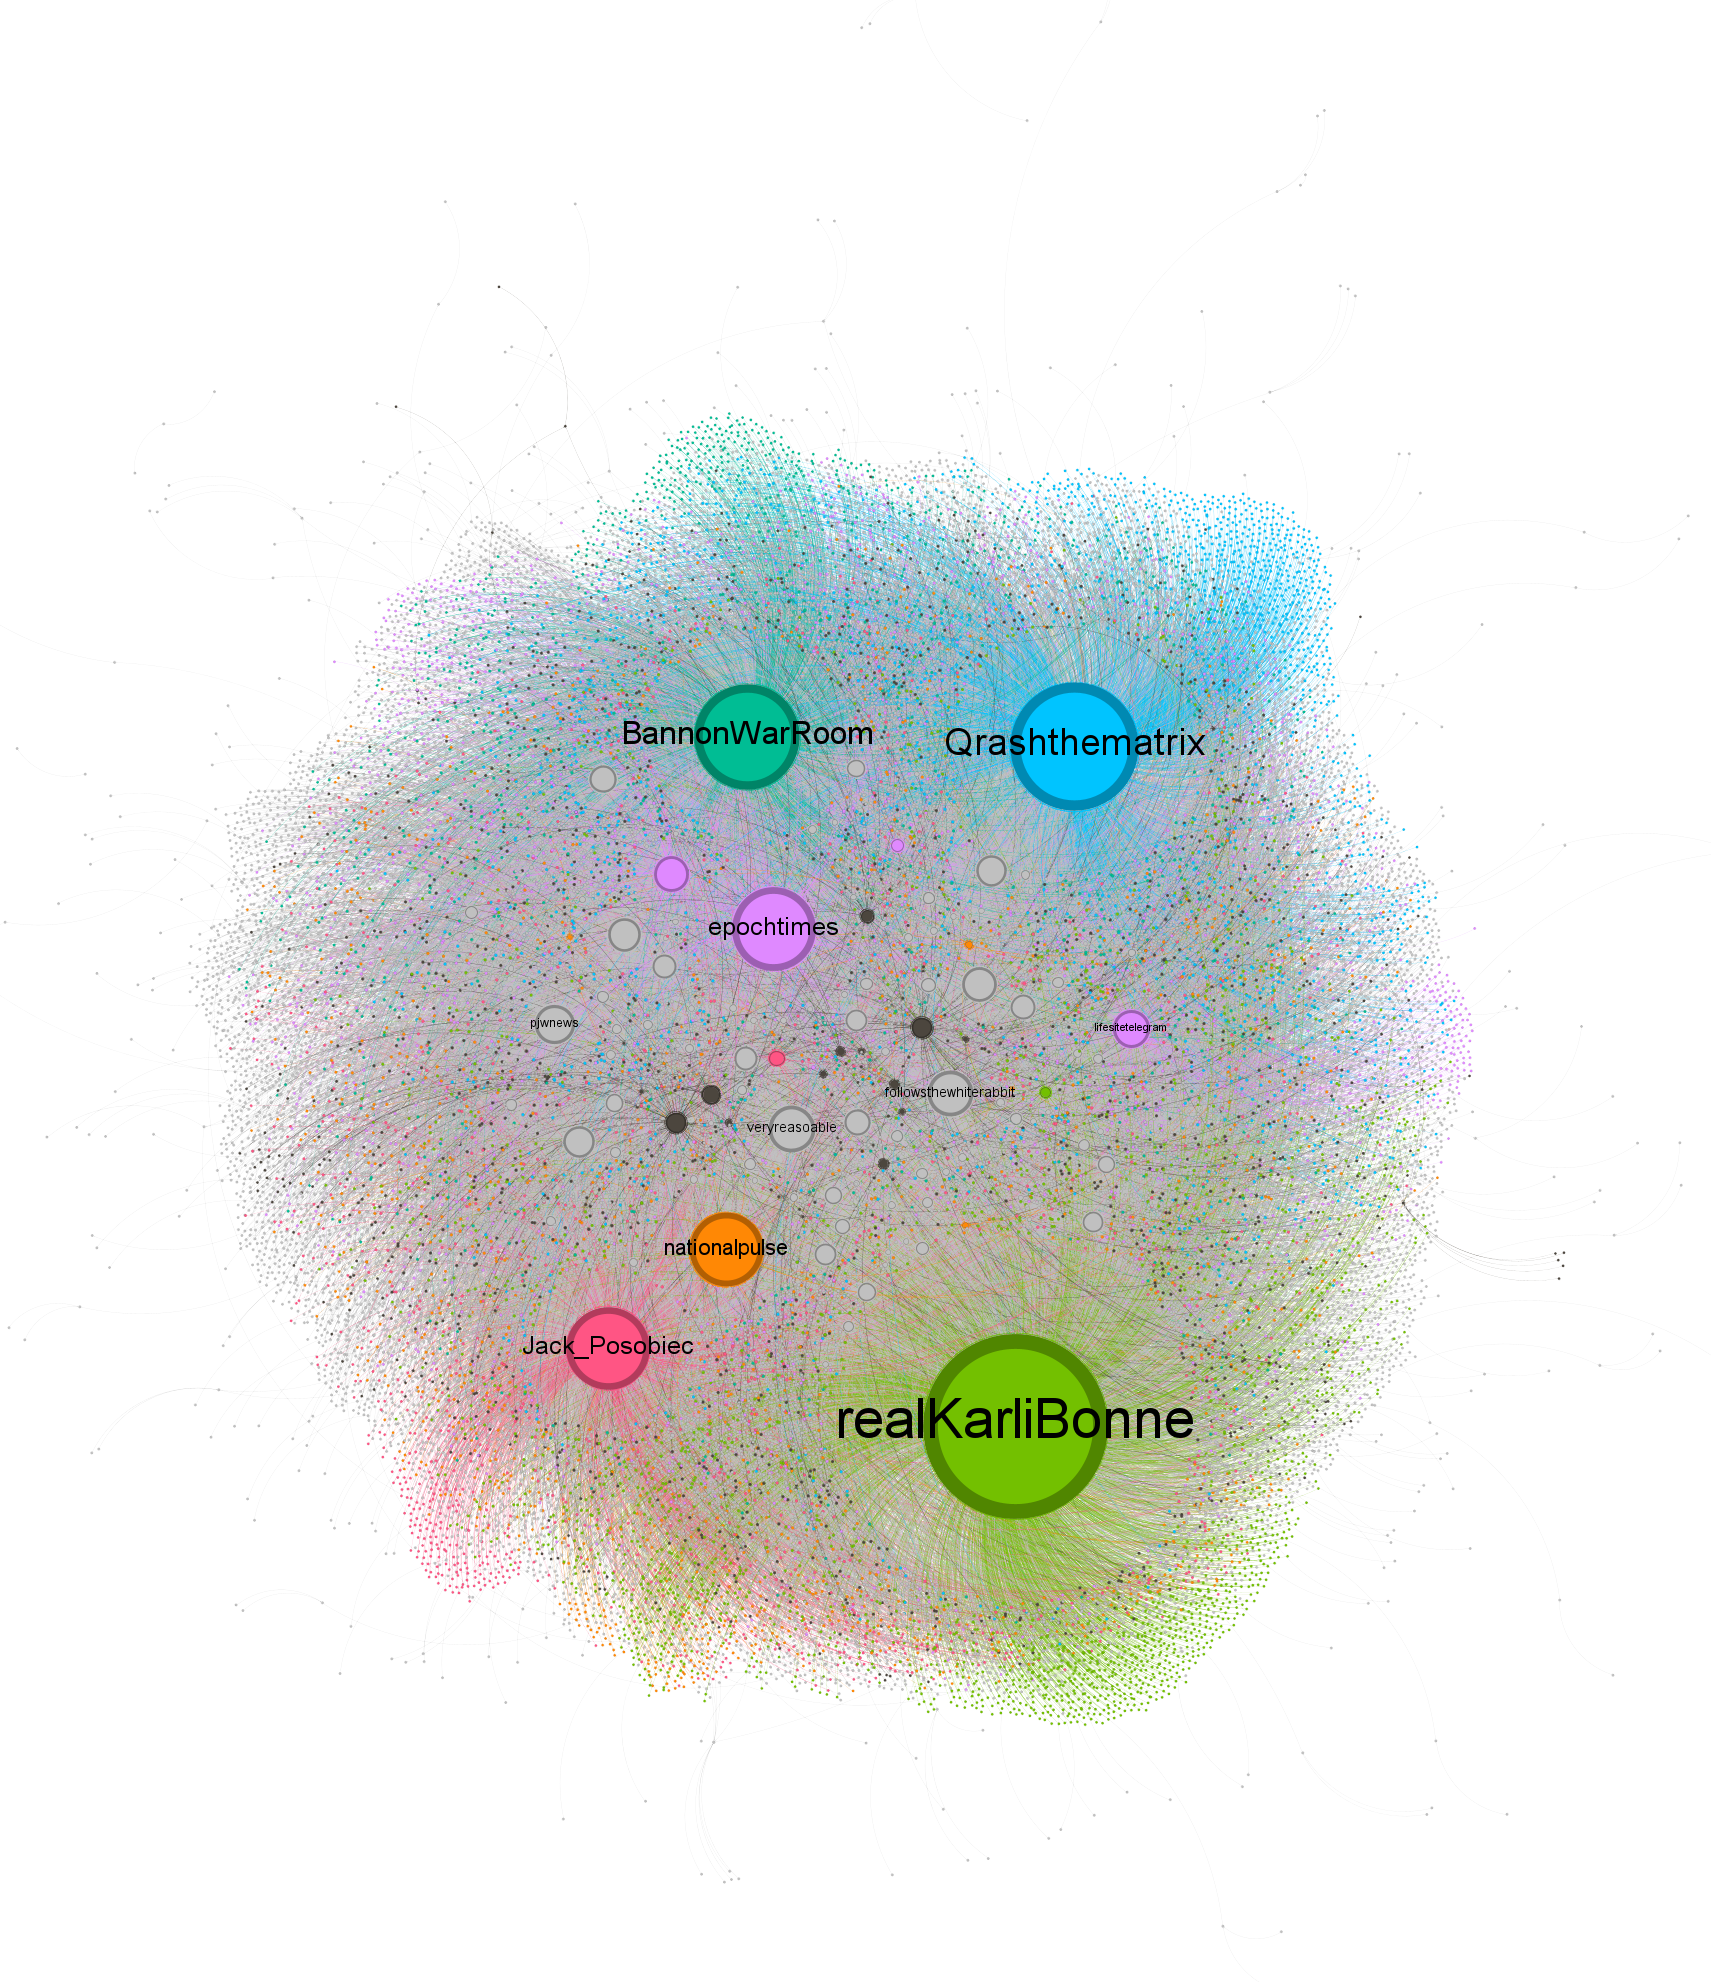
\includegraphics[width=0.8\textwidth]{immagini/graph}
	\end{figure}
	\subsubsection{Grafo non orientato}
	\subsection{Analisi dei grafi}
	\subsubsection{Analisi del grafo orientato}
	Il seguente codice implementa un’analisi strutturale sul grafo orientato e esportato in formato \textbf{.graphml}. \\Esso utilizza librerie Python come \textbf{NetworkX} per calcoli di metriche topologiche avanzate e \textbf{Pandas} per l’organizzazione e l’esportazione dei risultati. \\ Il grafo viene analizzato attraverso misure di centralità e metriche di rete. \\Di seguito è riportata una spiegazione dettagliata:
		\begin{itemize}[label=\ding{109}] 
		\item \textbf{Caricamento del grafo:}\\
		Il grafo viene caricato utilizzando il metodo \textbf{nx.read\_graphml}, che importa dati strutturati in formato \textbf{.graphml}. Una volta caricato, vengono stampate informazioni generali sulla rete, come il numero di nodi e di archi:
		\begin{lstlisting}
		print("Grafo caricato con successo. Numero di nodi:", graph.number_of_nodes(), "Numero di archi:", graph.number_of_edges())
		\end{lstlisting}
		Questo consente una verifica preliminare per assicurarsi che i dati siano stati importati correttamente.
		\item \textbf{Filtraggio dei nodi "channel":}
		Il codice filtra i nodi con un \textbf{attributo "type" pari a "Channel"}, utilizzando una lista comprensione:
		\begin{lstlisting}
		channels = [node for node in graph.nodes if graph.nodes[node].get("type") == "Channel"]
		\end{lstlisting}
		Questa operazione seleziona un sottoinsieme specifico del grafo, cosi da poter focalizzare l'analisi su canali Telegram piuttosto che su altri tipi di nodi. \\Il numero totale di nodi selezionati viene stampato per trasparenza.
		\item \textbf{Calcolo delle metriche di centralità:}
		\begin{itemize}
			\item \textbf{Degree:}\\
			Il grado rappresenta il numero di connessioni di un nodo ed è calcolato senza considerare eventuali pesi sugli archi:
			\begin{lstlisting}
			degree_dict = dict(graph.degree(channels))
			\end{lstlisting}
			Questa metrica è utile per identificare nodi altamente connessi all'interno della rete.
			\item \textbf{Betweeness Centrality:}\\
			Utilizzando l'algoritmo ottimizzato di Brandes, il codice misura quanto un nodo si trovi su percorsi più brevi tra coppie di altri nodi.\\ Questo indica l'importanza del nodo come intermediario:
			\begin{lstlisting}
			betweenness_dict = nx.betweenness_centrality(graph, normalized=True, endpoints=False)
			\end{lstlisting}
			L'opzione \textbf{normalized=True} assicura che i valori siano scalati rispetto alla dimensione del grafo.
			\item \textbf{Closeness Centrality:}\\
			Questa metrica misura quanto un nodo sia vicino a tutti gli altri nodi della rete, in termini di distanza geodetica:
			\begin{lstlisting}
			closeness_dict = nx.closeness_centrality(graph)
			\end{lstlisting}
			\item \textbf{Authority Score:}\\
			Se il grafo è orientato, viene calcolata l'authority di ciascun nodo utilizzando l'algoritmo HITS, che assegna punteggi in base alla qualità delle connessioni in entrata:
			\begin{lstlisting}
			_, authority_dict = nx.hits(graph, normalized=True)
			\end{lstlisting}
			Nel caso di grafi non orientati, l’authority viene impostata a zero, poiché Gephi non supporta il calcolo di questa metrica per grafi non diretti.
			\item \textbf{Eigenvector Centrality:}\\
			Questa metrica valuta l’influenza di un nodo in base all’importanza dei suoi vicini, calcolata iterativamente:
			\begin{lstlisting}
			eigenvector_dict = nx.eigenvector_centrality(graph, max_iter=1000, tol=1e-6)
			\end{lstlisting}
			Parametri come \textbf{max\_iter} e \textbf{tol} sono scelti per garantire la convergenza.
		\end{itemize}
		\item \textbf{Creazione dei risultati:}\\
		I risultati delle metriche vengono raccolti in una lista di dizionari, dove ciascun dizionario rappresenta un nodo e le relative metriche calcolate:
		\begin{lstlisting}
			results = []
			for node in channels:
			results.append({
				"Node": node,
				"Degree": degree_dict.get(node, 0),
				"Betweenness": betweenness_dict.get(node, 0),
				"Closeness": closeness_dict.get(node, 0),
				"Authority": authority_dict.get(node, 0),
				"Eigenvector": eigenvector_dict.get(node, 0),
			})
		\end{lstlisting}
		\item \textbf{Esportazione risultati:}\\
		I risultati vengono convertiti in un DataFrame di Pandas, una struttura dati tabellare, e salvati in \textbf{formato .csv}:
		\begin{lstlisting}
			df = pd.DataFrame(results)
			output_file = "channel_metrics_gephi.csv"
			df.to_csv(output_file, index=False)
		\end{lstlisting}
	\end{itemize}
	La fase successiva dell'analisi del grafi prevede che i dati derivati vengano elaborati ulteriormente per calcolare una nuova metrica chiamata \textbf{"tasso di apertura" (Openness)}.\\
	Questo processo consente di arricchire ulteriormente le informazioni estratte, aggiungendo una dimensione sintetica che combina diverse metriche di centralità per fornire una visione complessiva dell'importanza e della posizione strategica dei nodi della rete.\\
	Lo script si basa sue due file: il primo, \textbf{statpython.csv}, contiene i dati di base del grafo già processati e arricchiti con metriche di centralità; il secondo, \textbf{statpython\_with\_openness.csv}, viene generato dallo script ed include la nuova colonna "Openness" accanto alle metriche originali, ampliando cosi le possibilità di analisi successive.\\
	Il file\textbf{ statpython.csv} rappresenta una tabella con informazioni dettagliate per ogni nodo del grafo. Le colonne principali includono:
	\begin{itemize}[label=\ding{109}] 
		\item \textbf{Node:} identificativo univoco del nodo nella rete. Questo attributo consente di distinguere ciascun elemento analizzato, garantendo l'integrità dei collegamenti tra i dati originali e quelli derivati.
		\item \textbf{Degree:} numero di connessioni dirette che un nodo ha nella rete, una misura semplice ma fondamentale della sua interconnessione.
		\item \textbf{Betweeness:} misura dell'importanza di un nodo come intermediario nei percorsi brevi tra altri nodi, evidenziando il suo ruolo nel facilitare il flusso di informazioni.
		\item \textbf{Closeness:} rappresenta la vicinanza di un nodo a tutti gli altri nodi della rete, calcolata come l'inverso della somma delle distanze, una metrica utile per identificare nodi centrali.
		\item \textbf{Authority:} valore che indica l'autorevolezza del nodo basato sull'algoritmo HITS, particolarmente rilevante in grafi diretti dove l'influenza reciproca tra nodi gioca un ruolo cruciale.
		\item \textbf{Eigenvector:} centralità che misura l'influenza del nodo in base all'importanza dei nodi a cui è connesso, una metrica iterativa che considera il contesto globale della rete
	\end{itemize}
	Un esempio delle prime cinque righe di questo file è il seguente:
	\begin{lstlisting}
		Node, Degree, Betweenness, Closeness, Authority, Eigenvector
		1, 10, 0.02, 0.4, 0.3, 0.8
		2, 5, 0.01, 0.35, 0.2, 0.7
		3, 8, 0.03, 0.38, 0.25, 0.75
		4, 6, 0.015, 0.37, 0.22, 0.72
		5, 7, 0.02, 0.36, 0.24, 0.73
	\end{lstlisting}
	Questa struttura garantisce la chiarezza e la coerenza necessarie per operazioni successive di analisi e calcolo.\\
	Lo script inizia caricando i dati da \textbf{statpython.csv} utilizzando la \textbf{libreria pandas}, un potente strumento per la manipolazione di dati strutturati.\\ 
	Dopo aver caricato i dati, verifica che le colonne necessarie siano presenti, garantendo che il dataset sia completo e conforme ai requisiti dell'analisi:
	\begin{lstlisting}
		file_path = 'statpython.csv'
		df = pd.read_csv(file_path)
		required_columns = ["Node", "Degree", "Betweenness", "Closeness", "Authority", "Eigenvector"]
		if not all(col in df.columns for col in required_columns):
		raise ValueError(f"Il file CSV deve contenere le seguenti colonne: {', '.join(required_columns)}")
	\end{lstlisting}
	Se una delle colonne mancasse, lo script interromperebbe l'esecuzione con un messaggio di errore chiaro, assicurando un controllo di qualità sui dati in ingresso.\\
	Per rendere comparabili le diverse metriche, lo script utilizza il metodo \textbf{MinMaxScaler} di \textbf{sklearn} per scalare i valori nel range [0,1].\\
	Questa normalizzazione è essenziale per eliminare eventuali disparità dovute a scale diverse nelle metriche originali e garantire che ogni metrica contribuisca equamente al calcolo successivo:
	\begin{lstlisting}
		metrics = ["Degree", "Betweenness", "Closeness", "Authority", "Eigenvector"]
		scaler = MinMaxScaler()
		normalized_metrics = scaler.fit_transform(df[metrics])
	\end{lstlisting}
	Il risultato è una matrice in cui ogni valore rappresenta una versione scalata del corrispondente valore originale, uniformando l'importanza relativa di ciascuna metrica.\\
	La metrica \textbf{"Openness"} viene calcolata come la media aritmetica delle metriche normalizzate per ogni nodo.\\
	Questo approccio aggrega informazioni complesse in un unico valore, semplificando l'identificazione di nodi che mostrano una combinazione equilibrata di centralità e influenza:
	\begin{lstlisting}
		df["Openness"] = normalized_metrics.mean(axis=1)
	\end{lstlisting}
	Il risultato è una nuova colonna aggiunta al dataset, che fornisce un'indicazione sintetica ma potente del ruolo globale del nodo nella rete analizzata.\\
	Il file aggiornato, contenente la nuova colonna "Openness", viene salvato in un nuovo file CSV. \\Questa operazione consente di conservare i dati elaborati in un formato facilmente condivisibile e compatibile con ulteriori analisi:
	\begin{lstlisting}
		output_file_path = "statpython_with_openness.csv"
		df.to_csv(output_file_path, index=False)
	\end{lstlisting}
	Le prime cinque righe del file generato appaiono così:
	\begin{lstlisting}
		Node, Degree, Betweenness, Closeness, Authority, Eigenvector, Openness
		1, 10, 0.02, 0.4, 0.3, 0.8, 0.508
		2, 5, 0.01, 0.35, 0.2, 0.7, 0.432
		3, 8, 0.03, 0.38, 0.25, 0.75, 0.488
		4, 6, 0.015, 0.37, 0.22, 0.72, 0.465
		5, 7, 0.02, 0.36, 0.24, 0.73, 0.482
	\end{lstlisting}
	Questa tabella arricchita permette di ottenere informazioni preziose in modo rapido ed efficiente.\\
	Questo approccio permette di integrare informazioni complesse in un formato più facilmente interpretabile, utile per identificare nodi particolarmente influenti o strategici nella rete. \\Inoltre, la combinazione dei due file consente una pipeline analitica ben definita, in cui ogni fase aggiunge un livello di approfondimento, migliorando la comprensione della struttura e delle dinamiche della rete.
	\subsubsection{Analisi del grafo non orientato}
	\subsection{Analisi dei risultati}
	\section{Clustering}
	\section{Conclusione e valutazione finale del team}
	\subsection{Sintesi dei risultati}
	
	
\end{document}